\begin{center}
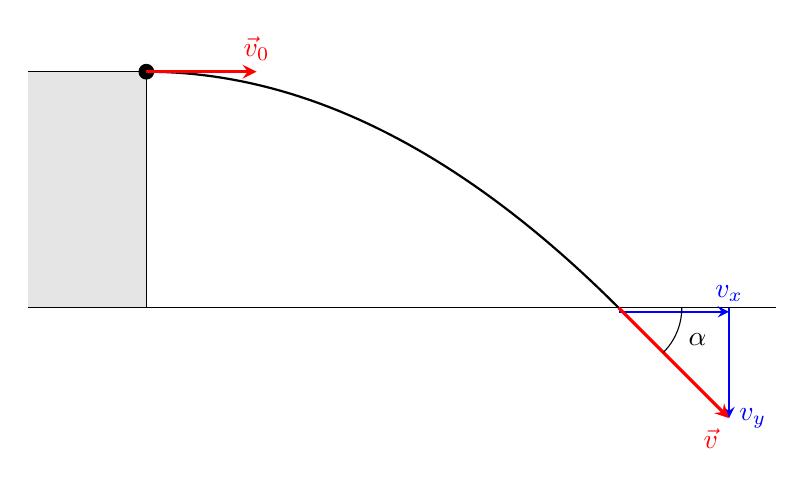
\begin{tikzpicture}[>=stealth]
 \fill[gray!20] (-1.5,0) rectangle (0,3);
 \draw (-1.5,3) -- (0,3) -- (0,0);
 \draw (-1.5,0) -- (8,0);
 \draw[thick, domain=0:6, samples=50] plot (\x, {3-\x*\x/12});
 \fill (0,3) circle (0.1);
 \draw[->, very thick, red] (0,3) -- (1.4,3) node[above] {$\vec v_0$};
 \draw[->, thick, blue] (6,-0.05) -- (7.4,-0.05) node[above] {$v_x$};
 \draw[->, thick, blue] (7.4,0) -- (7.4,-1.4) node[right] {$v_y$};
 \draw[->, very thick, red] (6,0) -- (7.4,-1.4) node[below left] {$\vec v$};
 \draw (6.8,0) arc (0:-45:0.8);
 \node at (7.0,-0.4) {$\alpha$};
\end{tikzpicture}
\end{center}

Die horizontale Teilgeschwindigkeit bleibt während des ganzen Flugs gleich der Anfangsgeschwindigkeit, $v_x = v_0$. Die vertikale Teilgeschwindigkeit wächst wie beim freien Fall, beim Aufprall ist $v_y = g\,t$. Für den Aufprallwinkel gilt
\begin{align}
 \tan\alpha &= \frac{v_y}{v_x} = \frac{g\,t}{v_0}
\end{align}
und damit
\begin{align}
 v_0 &= \voF \\
   &= \frac{\gE\cdot\tfl}{\tan\left(\alO\right)} \\
   &= \vo \approx \result{\voP{0}{2}}
\end{align}
